\section{Nuclear fission}
\label{sec:fission}
Nuclear fission is the process by which a nucleus splits into two -- sometimes three -- nuclei, whether spontaneously or when induced by a reaction.
The physics that governs nuclear fission is that of a many-body, large-amplitude collective mode that gradually elongates the nuclear shape until the so-called \textit{fission barrier} is surmounted and the energetically favoured path leads the nucleus to fragment. In Figure~\ref{fig:fission_barrier}, a graphical representation of the fission path and corresponding barrier is shown.

\begin{figure}[h]
    \centering
    \includegraphics[width=0.8\textwidth]{Images/mocca_barrier.png}
    \caption[Fission path of $^{226}$Ra, with different imposed spatial constraints.]{Fission path of $^{226}$Ra, blue lines indicate axial octupole configurations, black lines indicate axial quadrupole and parity conserving configurations, red lines indicate triaxial, parity conserving configurations. Figure taken from~\cite{Ryssens2016_MOCCa}.}
    \label{fig:fission_barrier}
\end{figure}

Although the basic idea of a nucleus dividing into two pieces may appear simple, the underlying dynamics is remarkably rich and involves several stages. Historically, the first theoretical interpretation of fission was given by Bohr and Wheeler in 1939 \cite{BohrWheeler1939_PR56_426}, who formulated the liquid-drop model description and introduced the concept of the fission barrier, determined by the competition between Coulomb repulsion and surface tension. Their framework already suggested that nuclei may experience intermediate configurations, multiple saddle points, and shape isomerism along the fission path.

Subsequent developments incorporated more detailed descriptions of the collective degrees of freedom and the role of shell effects, leading to the recognition that the fission landscape is often characterised by multiple barriers, intermediate minima, and highly deformed transition states \cite{Strutinsky1967_NPA95_420,Brack1972_RMP44_320}. Modern microscopic approaches, based on energy-density functionals, have further clarified that fission dynamics involves a sequence of slow, dissipative shape evolutions, interspersed with possible gamma-decay pathways, and culminating in the formation of two (or more) pre-fragments connected by a narrowing neck. As the system evolves beyond the outer saddle, exotic spatial configurations appear, and the fragments themselves may exhibit deformation or even reflection asymmetry before scission. A visual representation of the overall fission process is shown in Figure~\ref{fig:fission}.


\begin{figure}[h]
    \centering
    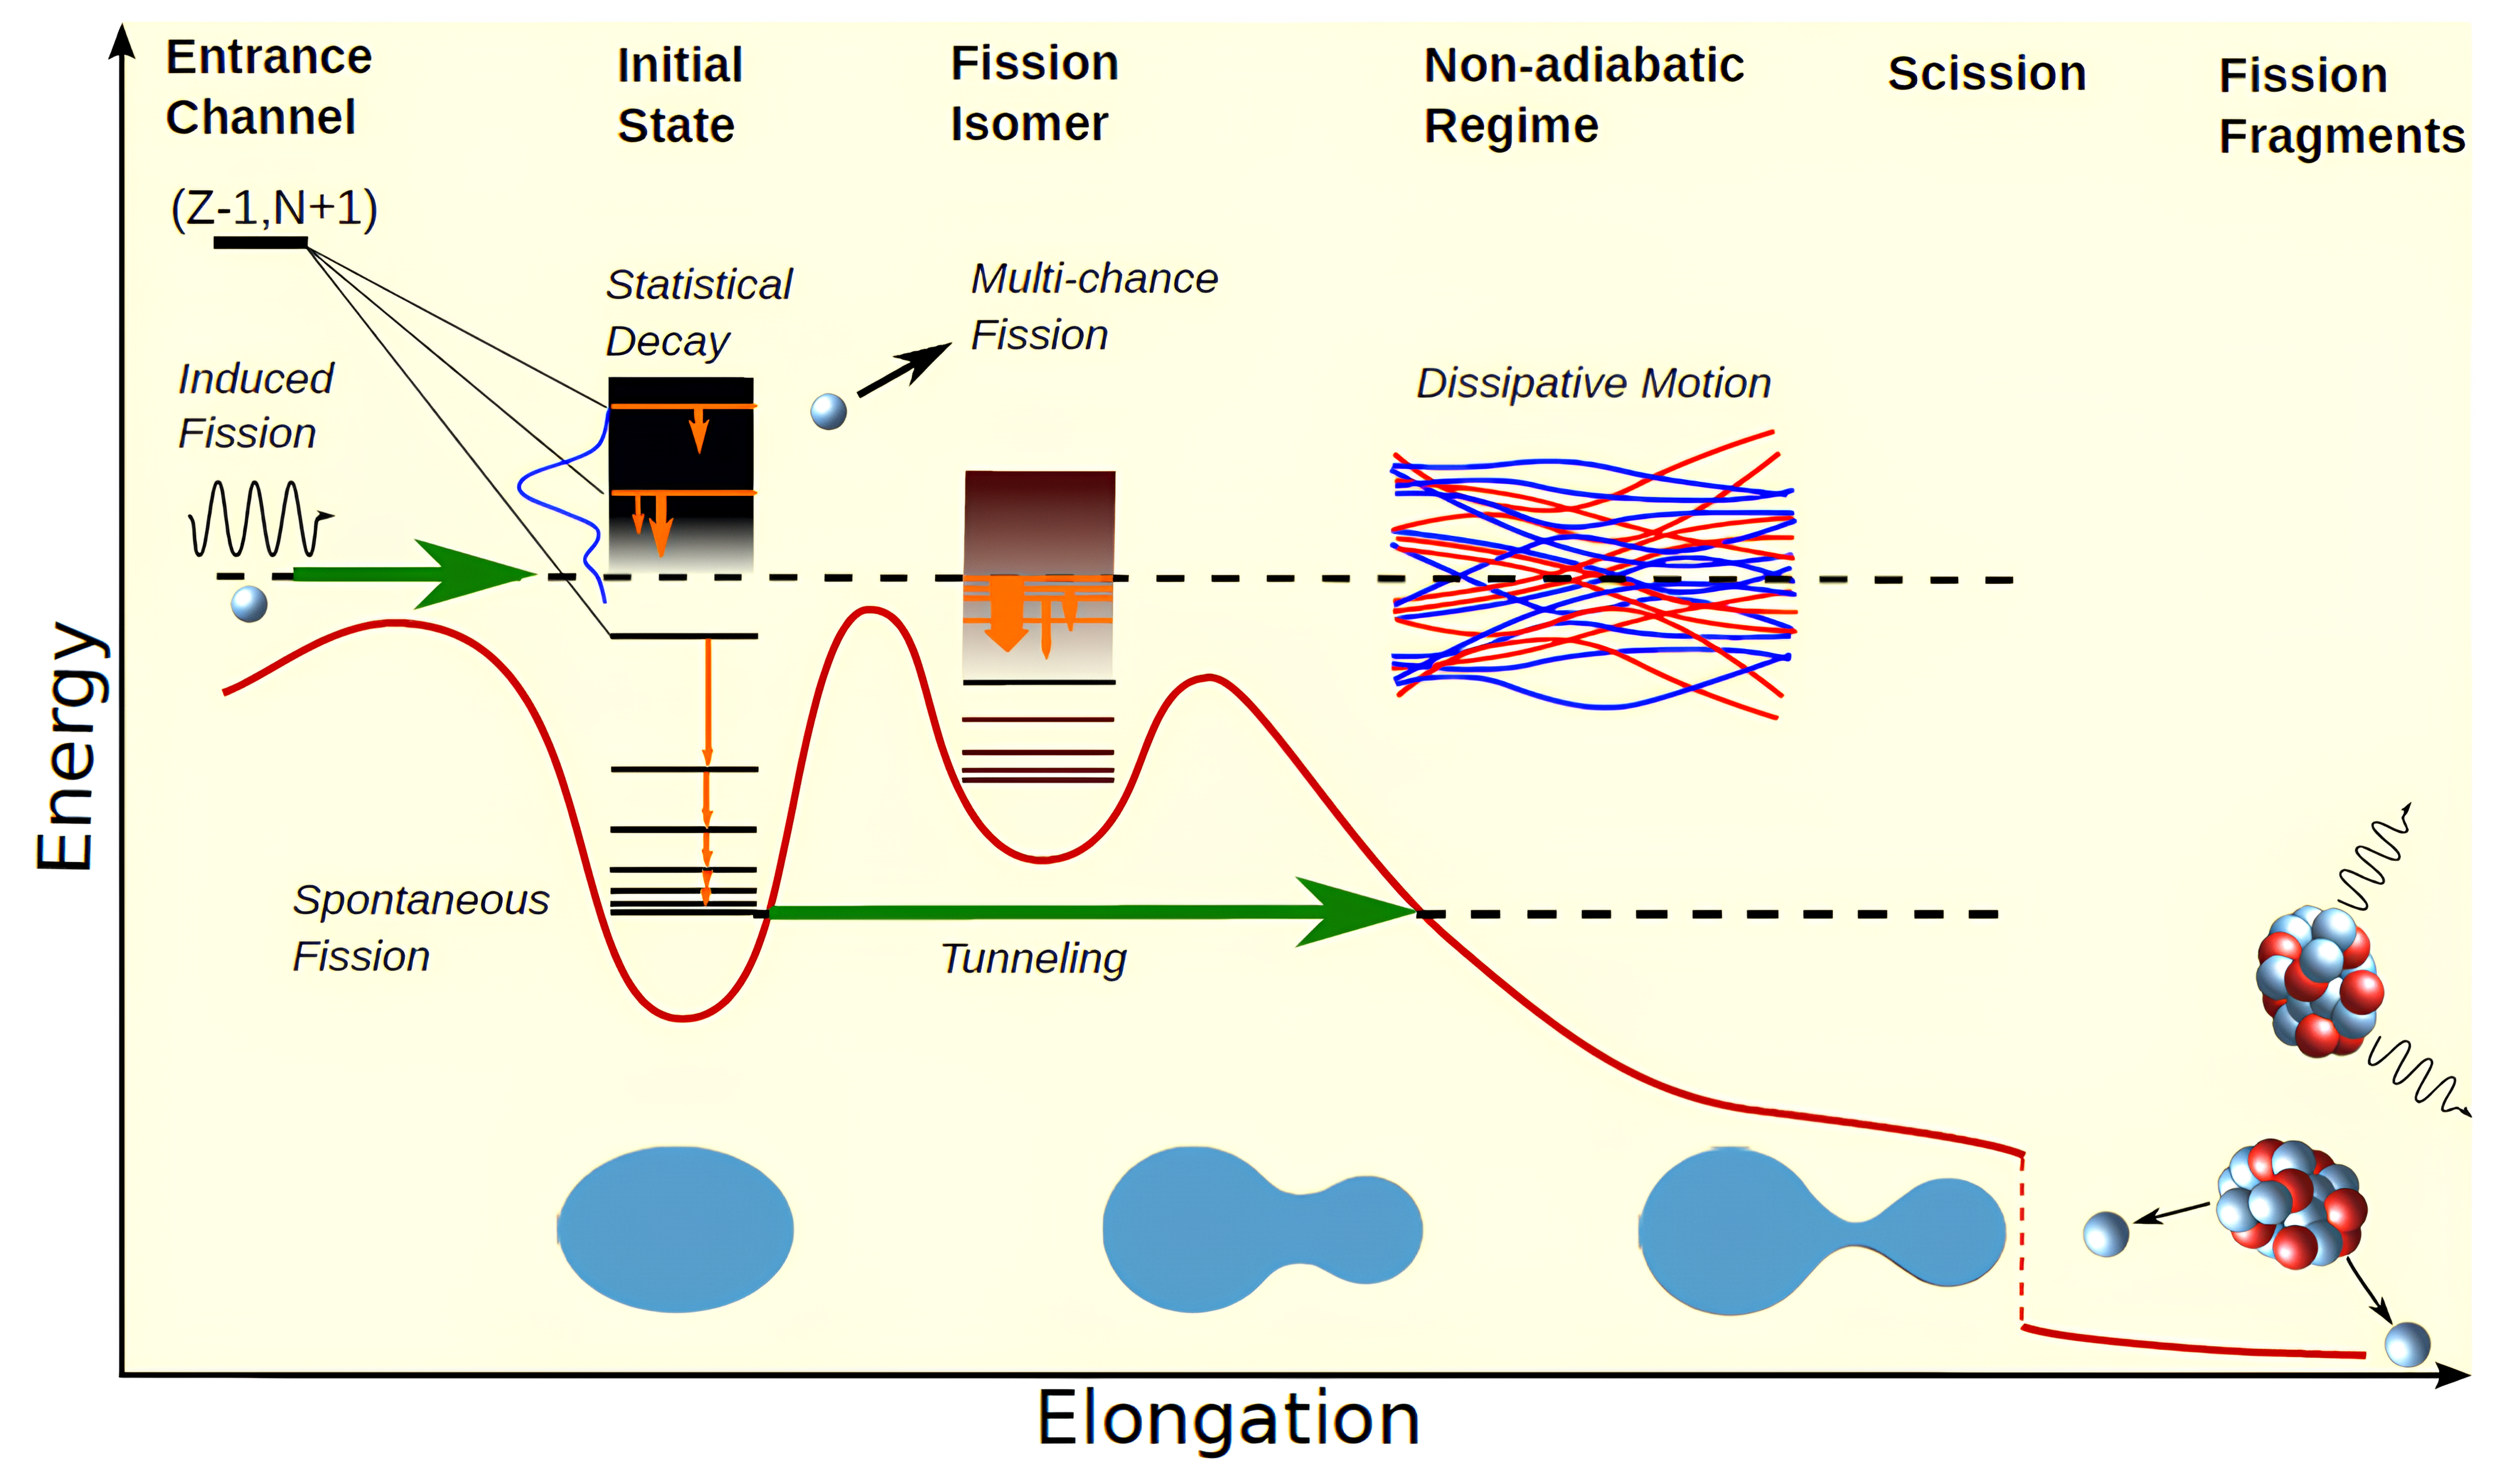
\includegraphics[width=0.85\textwidth]{Images/fission.png}
    \caption[Visual representation of the fission process.]{Visual representation of the fission process. Figure taken from~\cite{Bender2020}.}
    \label{fig:fission}
\end{figure}

\subsubsection{Spontaneous fission model}
It should be ovious that a formal treatment of deformations and collective modes is necessary to give a theoretical description of fission reactions. We can derive a simple spontaneous fission model by studying the effect of an axial quadrupole deformation on the semiempirical mass formula \ref{eq:semf}.

Let us assume that the nuclear radius may be expanded, as previously done in Section~\ref{sec:deformations}, as
\begin{equation}
    R = R_0[1+\alpha_{20}Y_{20}].
\end{equation}
Assuming the nuclear volume is conserved across the fission path, the volume energy will not change. As for the surface energy, its variation can be expressed at the lowest order in $\alpha_{20}$ as
\begin{equation}
    \Delta E_\text{surf} = E_\text{surf}
    -E_{0,\text{surf}} = E_{0, \text{surf}}\frac 2 5 \alpha_{20}^2.
\end{equation}
Regarding the Coulomb energy, the variation is given by
\begin{equation}
    \Delta E_\text{coul} = E_\text{coul} - E_{0, \text{coul}} = -E_{0, \text{coul}}\frac 1 5 \alpha_{20}.
\end{equation}
Since the neutron and proton numbers does not change, the surface and Coulomb energies are the only contributions to the total energy difference. We can write
\begin{equation}
    \label{eq:fission_semf}
    \Delta E = \frac 2 5 \alpha_{20}^2 a_s A^{2/3}- \frac 1 5 \alpha_{20}^2 a_c Z^2 A^{-1/3},
\end{equation}
if we set Equation~\eqref{eq:fission_semf} to zero, we get, other than the undeformed solution for $\alpha_{20}=0$, 
\begin{equation}
    \frac{ Z^2}{A} = \frac{2 a_s}{a_c},
\end{equation}
where the ratio $2a_s/a_c$ amounts to $\approx 50$ in typical parametrisations of the SEMF. Equation~\eqref{eq:fission_semf}, shows that for values of the so called \textit{fissility parameter} $Z^2/A$ larger than $50$, the energy change becomes negative, favouring a configuration in which the nucleus fragments due to the spontaneous fission.

\subsubsection{Pairing correlations in fission}
Pairing correlations are fundamental to quantitatively describe the fission process and the difference between fissile and fissionable materials.
As a general example, applicable to heavy nuclei in the actinide region, we can examine the difference between $^{235}$U and $^{238}$U in their fission induced by a thermal neutron.
The fission barrier height for $^{239}$U is $\approx 5.5$ MeV, while for $^{236}$U it is $\approx 5.3$ MeV. Although the diffence is small, when $^{235}U$ captures a thermal neutron the latter is able to fission while the former is not when $^{238}$U captures a thermal neutron. This is due to the stronger pairing correlations in even nuclei than in odd nuclei, as the compound nucleus binding energy is higher when the neutron and/or proton number is even, favouring fission.

The presence of pairing correlations is also fundamental when quantitatively describing the evolution from the ground state to the scission. Pairing correlations allow the nuclear density to take on many different additional configurations, as the fission barrier is traversed in a superposition of these shapes, as explained more in depth in Section~\ref{sec:microscopic_fission}, the fragmentation happens more easily \cite{FissionPathPairing}.